\chapter{Software and Firmware Development}

\graphicspath{{./Figures/Firmware and Testing/}}
This chapter discusses the software and firmware development for the robot.
Providing a through explanation of the software and firmware that form the backbone of the robot's functionality.
it outlines the process of developing, integrating, and management of these systems, emphasizing the importance of each component and its role in the overall system.
The chapter stands as a reference to the complexity and sophistication of involved in developing advanced robotic systems, where every layer of the software and firmware stack is carefully designed and implemented to ensure the proper operation of the robot.

%\begin{itemize}
%	\item Overview of the chapter's content and its significance in the context of the overall project.
%	\item Briefly state the objectives of firmware development and testing procedures.
%\end{itemize}
\newpage
\section{Overview}
%figure for Hardware diagram
\begin {figure}[h]
\centering
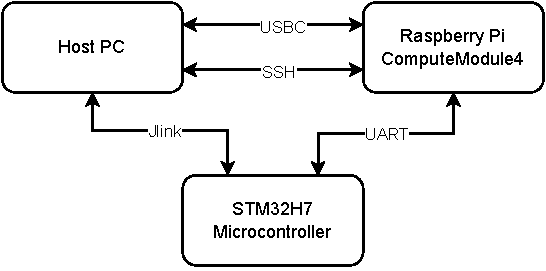
\includegraphics[width=0.8\textwidth]{Hardware diagram}
\caption{Hardware diagram}
\label{fig:Hardware}
\end {figure}

As shown in Figure\ref{fig:Hardware}, system architecture is divided into three main parts: microcontroller firmware, raspberry pi software, and host pc software.
The microcontroller firmware is responsible for controlling the robot's actuators and sensors.
The raspberry pi software is responsible for high-level tasks of the robot.
The host pc software is responsible for

\section{Microcontroller Firmware}
%Development Environment: Mention that the firmware is developed in C and C++, and highlight the use of FreeRTOS for task scheduling and management.
%state estimation
The microcontroller firmware is responsible for controlling the robot's actuators and sensors.
As outlined in the electrical design Chapter, STM32H7 microcontroller is the main controller for the robot.
The firmware is written in C language, with some parts written in C++.
FreeRTOS is used as the real-time operating system for the microcontroller for task scheduling and management.

%Feedback Control: Explain the firmware’s role in real-time feedback control, focusing on balancing and dynamic adjustments.

Feedback control is implemented in the firmware to control the robot's actuators.
The feedback control is implemented using different control algorithms.
Balancing the robot in different configurations is the main goal of the feedback control.
State estimation is implemented in the firmware to estimate the robot's state and provide feedback to the control algorithms that generate the control signals for the actuators.
Time critical functions are implemented in the firmware to ensure the real-time performance of the robot.
These functions include the control loop for balancing the robot and some other functions that are time-critical such as safety protocols.
The safety protocols are implemented to ensure the safety of the robot and the user.
The safety protocols include the emergency stop for the motors in case of high current draw or high temperature.
Such protocols ensure, for example, that the robot will not accelerate to a high speed and crash into an object.

%Filtering : Detail the filtering techniques .
%Motor Control and Sensor Integration: Describe the mechanisms for motor control and sensor data processing.
The microcontroller firmware is responsible for different tasks that ensure the robot's proper operation.
Tasks such as reading the sensors and filtering the sensor data are implemented in the firmware.
The firmware is also responsible for controlling the motors and real time monitoring feedback from the motors to verify that the motors have reached the desired state as per the last control signal sent to the motors.


\section{Raspberry Pi Software}
%Development Environment: Mention that the software is developed in Python, and highlight the use of ROS for task scheduling and management.
The raspberry pi software is an important part of the robot's software.
It is written in Python and deals with the high-level tasks of the robot.
The raspberry pi allows wireless SSH connection to the robot, which allows the user to change the control parameters or control the robot using a joystick.
The wireless connection allows different modifications to the robot's software without the need to connect the microcontroller to the computer as long as the raspberry pi and the pc are connected to the same network.
The raspberry pi software is responsible for highr complex tasks such as speed control and position control.
These tasks are not time-critical and can be implemented in the raspberry pi software.
Then it can be interpreted by the microcontroller firmware into a series of low-level control signals for the actuators.
Different applications such as navigation and mapping can be implemented in the raspberry pi software.
Image processing and computer vision can be a powerful tool for the robot to interact with its environment.

The raspberry pi software allows conducting experiments and collecting data from the robot.
The data acquired from the robot can be used to improve the robot's performance and control algorithms.
The raspberry pi software is provides an easy to use python interface for controlling the robot.


\section{Host PC Software}
%the third component is the software running on the host
%- controlling multiple robots
%- reading/writing parameters of individual robots
%- controlling the behavior of individual/multiple robots
%- deploying firmware to multiple robots
The host pc software is the third component of the robot's software.
It is responsible for controlling multiple robots.
It is also responsible for reading and writing parameters of individual or multiple robots.
The changes in the parameters influence the behavior of the robot.
The host pc software is also responsible for deploying firmware to multiple robots.
%IDE
\section{Integrated Development Environment}
STM32CubeIDE is used as the IDE for firmware development.
The STM32CubeIDE is based on the Eclipse IDE, which is an open-source IDE. The STM32CubeIDE allows clock configuration for the microcontroller.
The STM32Cube also generates the Makefile for the project, which is used to compile the firmware.
%figure for the Pinout & Configuration
\begin {figure}[h]
\centering
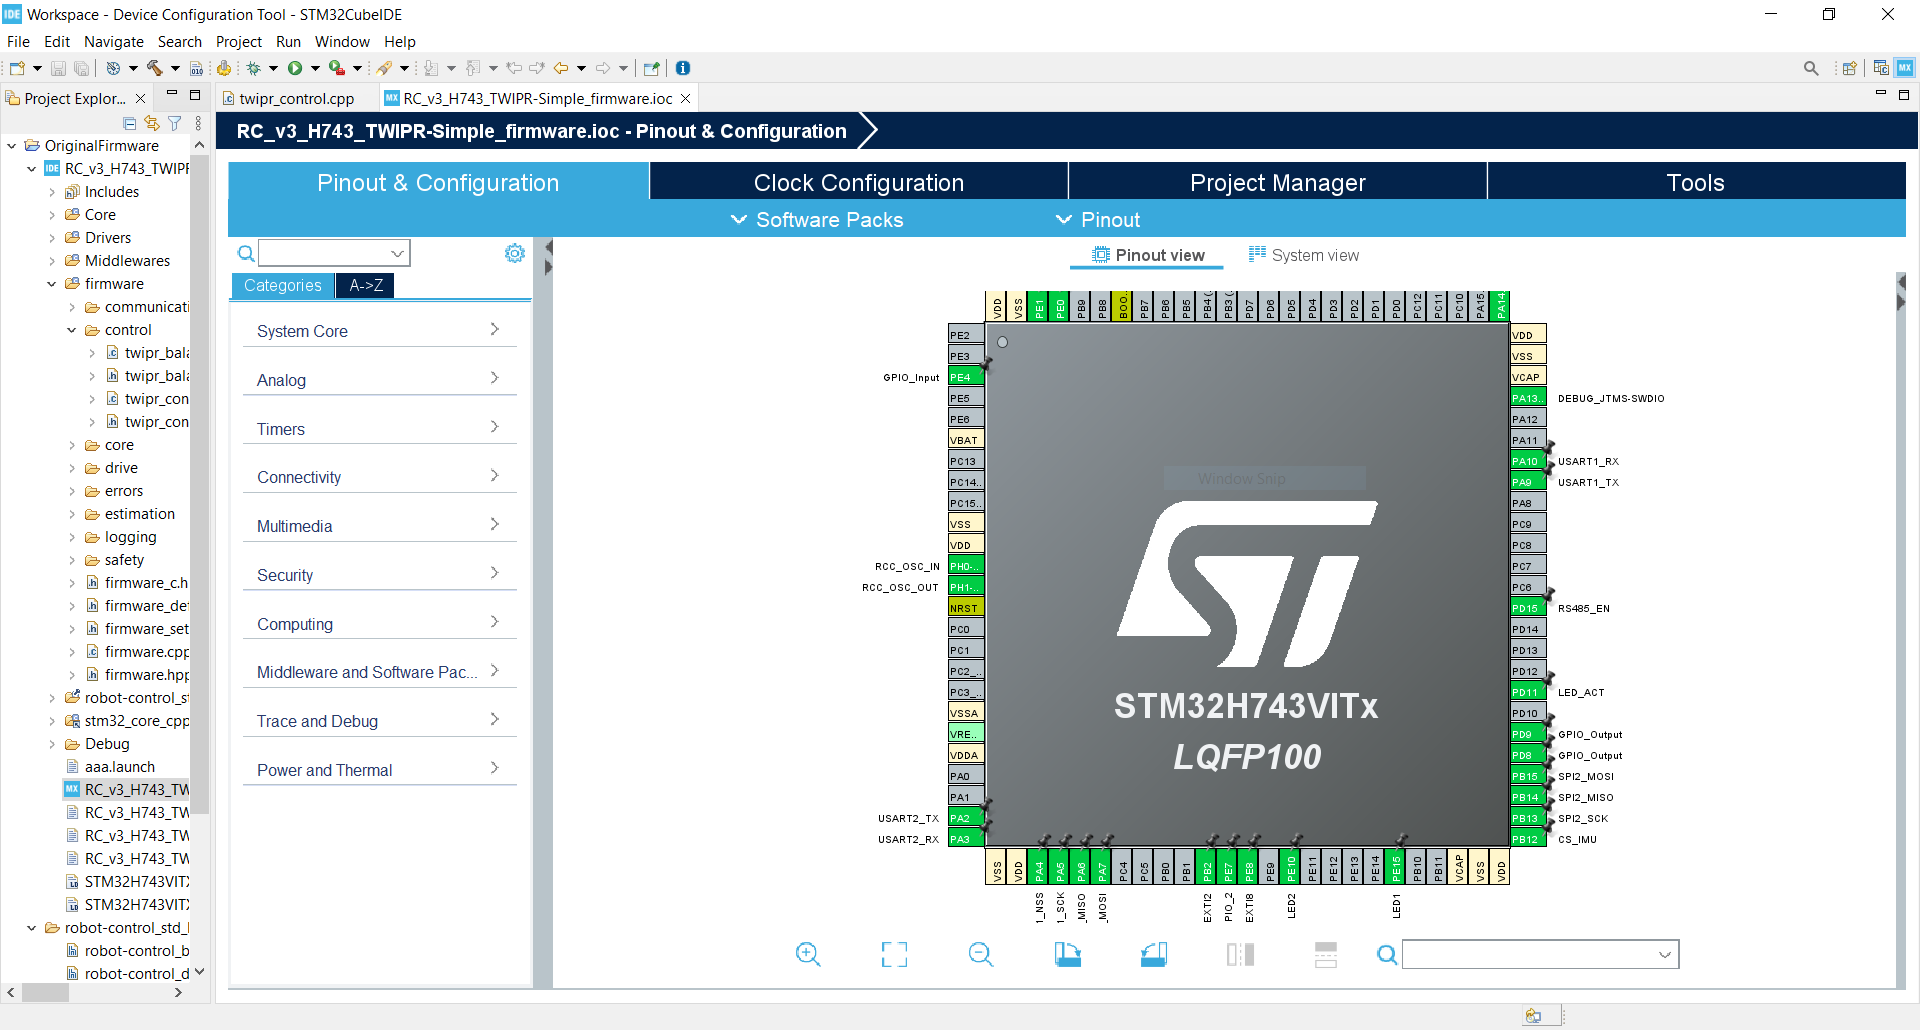
\includegraphics[width=.8\textwidth]{Pinout & Configuration}
\caption{Pinout \& Configuration}
\label{fig:Pinout}
\end {figure}

As shown in Figure \ref{fig:Pinout}, the STM32CubeIDE allows the user to configure the microcontroller peripherals, such as the GPIOs, timers, and UART. After configuring the microcontroller, the STM32CubeIDE generates the initialization code for the user.
%figure for the clock confugration
\begin {figure}[h]
\centering
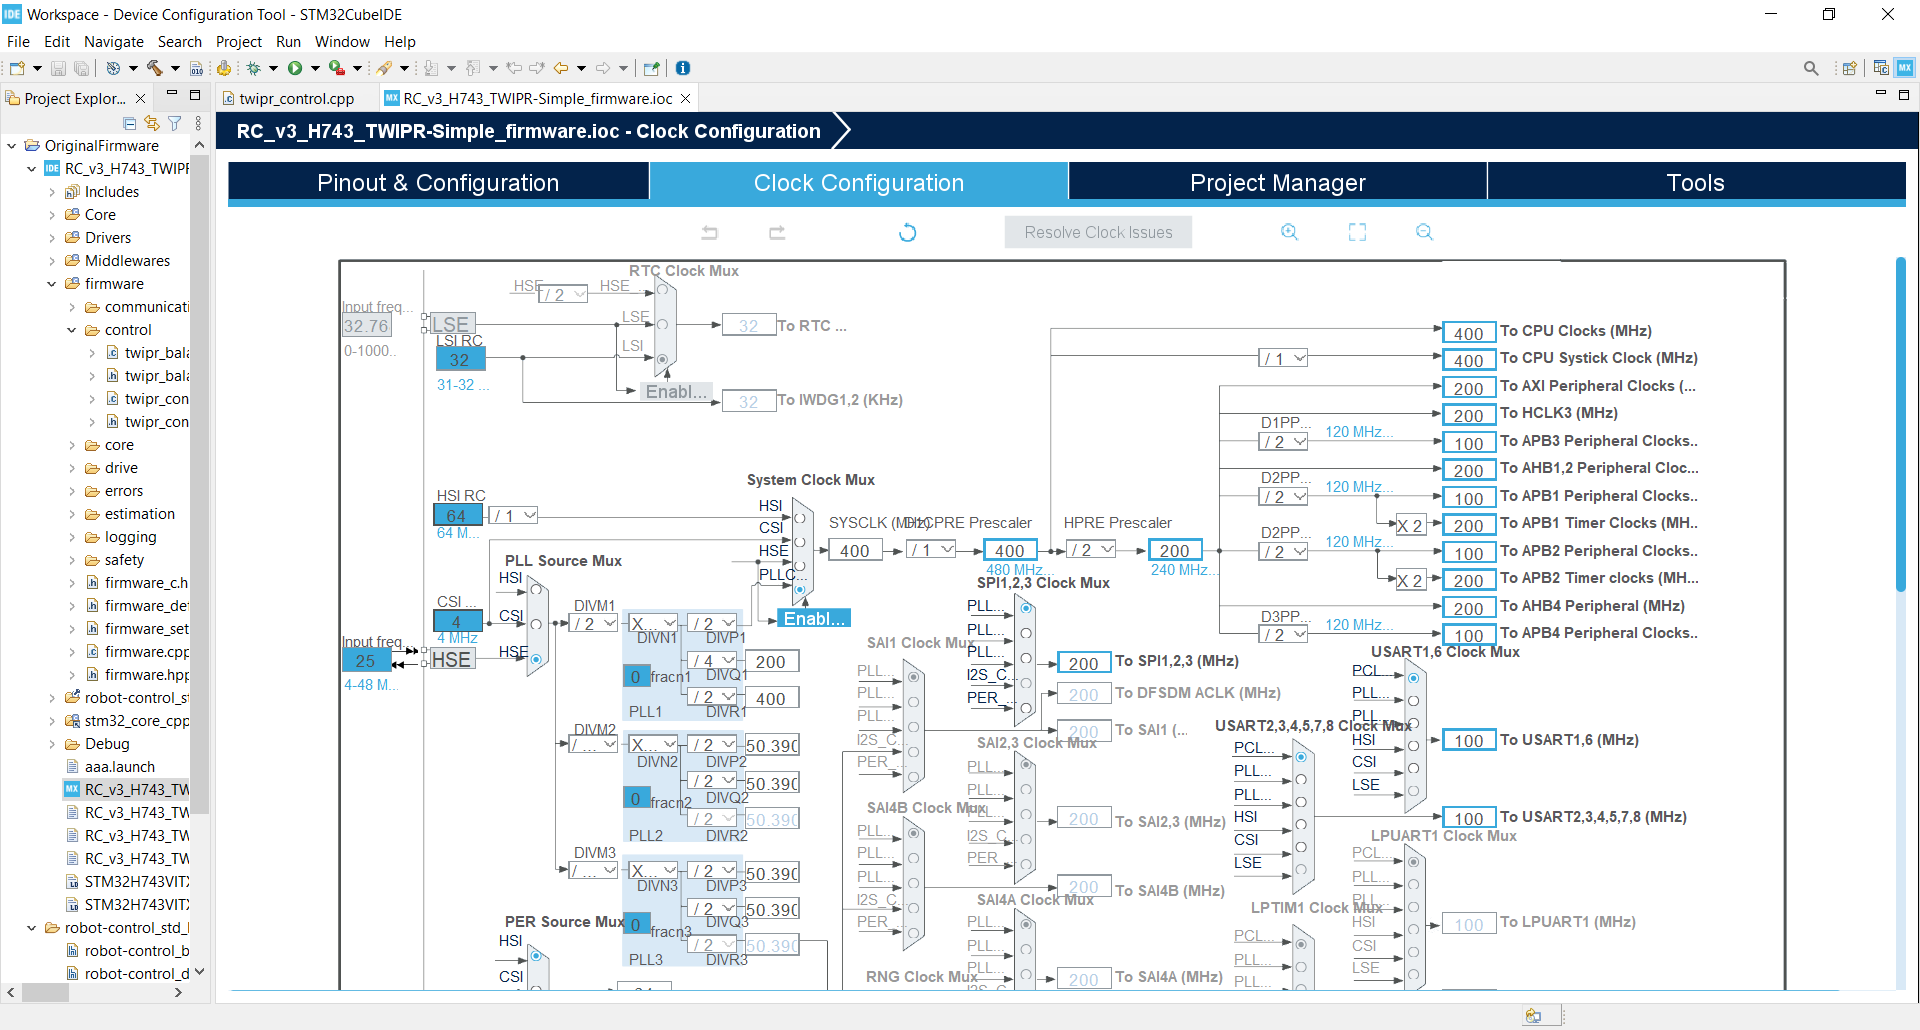
\includegraphics[width=.8\textwidth]{Clock Configuration}
\caption{Clock Configuration}
\label{fig:clock}
\end {figure}

The STM32CubeIDE allows clock configuration for the microcontroller as shown in Figure \ref{fig:clock}.



\section{Integration with Hardware}
The robot hub Board is used to connect the microcontroller to the sensors and actuators. It also provides the power supply for the microcontroller as well as acting as a carrier board for raspberry pi.
The robot hub board allows using the full potential of the microcontroller by providing the necessary connections.
%\begin{itemize}
%	\item Discuss how the firmware interacts with and controls the hardware components.
%	\item Explain any challenges encountered in integration and how they were resolved.
%\end{itemize}


\section{Debugging and Troubleshooting}
%\begin{itemize}
%	\item Discuss the process of debugging and troubleshooting encountered problems.
%	\item Explain how issues were diagnosed and resolved.
%\end{itemize}
%figure for Jlink
\begin {figure}[h]
\centering
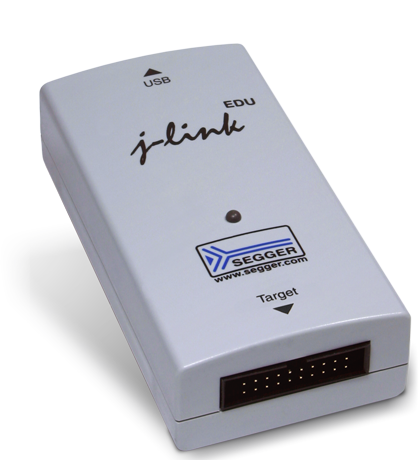
\includegraphics[width=0.3\textwidth]{jlink}
\caption{Jlink Debugger}
\label{fig:Jlink}
\end {figure}


Jlink s used to upload the firmware to the microcontroller.
As well as debugging the firmware.
The Jlink is a hardware debugger that connects to the microcontroller using the SWD interface.
The Jlink allows debugging breakpoints and stepping through the code.


